\documentclass[tikz]{standalone}
\usepackage{pgfplots}
\pgfplotsset{compat=1.15}
\usepackage{mathrsfs}
\usetikzlibrary{arrows,calc}
\usepackage{tkz-euclide}

\pagestyle{empty}

\definecolor{AngleClr}{rgb}{0,0.39215686274509803,0}
\definecolor{ShapeClr}{rgb}{0.6,0.2,0}
\definecolor{BlueClr}{RGB}{5,81,163}

\begin{document}

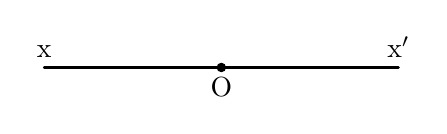
\begin{tikzpicture}[scale=.75]
\tkzSetUpLine[line width=1pt,color=black]
\tkzSetUpPoint[fill=black]

\tkzDefPoints{0/0/O,-3/0/x,3/0/x'}

\tkzDrawSegments[line width=1pt](x,x')

\tkzDrawPoints[size=3](O)
\tkzLabelPoint[below](O){$\rm O$}
\tkzLabelSegment[above,sloped,pos=0](x,O){$\rm x$}
\tkzLabelSegment[above,sloped,pos=0](x',O){$\rm x'$}


\end{tikzpicture}

\end{document}
